\documentclass[12pt, twoside]{article}
\usepackage[letterpaper, margin=1in, head=30pt, headsep=0.1in]{geometry}
\usepackage[english]{babel}
\usepackage[utf8]{inputenc}
\usepackage{amsmath}
\usepackage{amsfonts}
\usepackage{amssymb}
\usepackage{tikz}
\usetikzlibrary{quotes, angles}

\usepackage{graphicx}
\usepackage{enumitem}
\usepackage{multicol}

%\usepackage{pgfplots}
%\pgfplotsset{width=10cm,compat=1.9}
%\usepgfplotslibrary{statistics}
%\usepackage{pgfplotstable}
%\usepackage{tkz-fct}
%\usepackage{venndiagram}

\usepackage{fancyhdr}
\pagestyle{fancy}
\fancyhf{}
\renewcommand{\headrulewidth}{0pt} % disable the underline of the header
\raggedbottom
\newif\ifmeta
\metatrue %print standards and topics tags

\title{Math AI Worksheet Generator and Formative Assessment System}
\author{Chris Huson}
\date{January 2021}

%\fancyhead[RE]{\thepage}
%\fancyhead[RO]{\thepage \\ Name: \hspace{3cm}}
%\fancyhead[L]{BECA / Dr. Huson / 10th Grade Geometry\\* 7 June 2019}
%
%\begin{document}
%\subsubsection*{13.7 Homework: Cross sections, distance applications}
%\fancyhead[L]{BECA / Dr. Huson / Geometry 03-Volume+angle-bisectors\\* pset ID: 34}

\begin{document}

\subsubsection*{6.13 Density applications}
\begin{enumerate}

\item Do Now: Find the area of a triangle with base $b=12.5$ and height $h=8.4$. Use the Graspable Math activity linked above. Paste a cropped screenshot of the first problem here. It should look like the modelled solution below.
\begin{itemize}[label=$\square$]
  \item Copy expressions (drag the handle on the left of the formula)
  \item Substitute values (drag the variable onto the formula)
  \item Show/hide steps (show the substitution, final line, and key steps)
  \item Copy/paste screenshot: command-control-shift-4 (Mac)
\end{itemize}
\begin{flushright}
  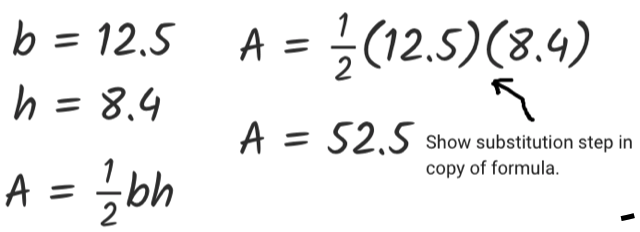
\includegraphics[width=8cm]{6-13-1_model-solution.png}
\end{flushright}

\newpage
\item Find the area of a semi-circle with radius $r=7.5$. Paste a cropped screenshot of the Graspable Math. Compare your format to the model solution.
\item \vspace{4cm}
\begin{flushright}
  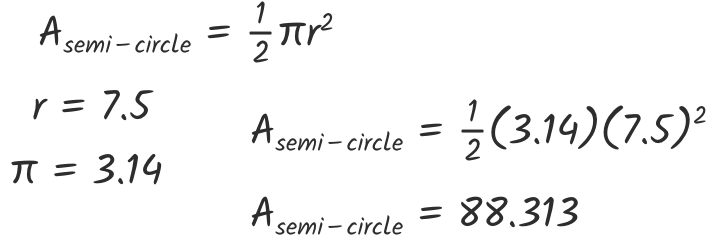
\includegraphics[width=10cm]{6-13-2-solution.png}
\end{flushright}

\newpage
\item Find the population density of Queens, New York. Paste a cropped screenshot of the Graspable Math. Make a copy of the formula and show the substitution step.
\vspace{4cm}
\begin{flushright}
  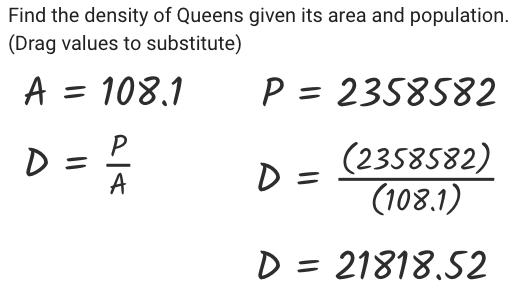
\includegraphics[width=9cm]{6-13-3-solution.png}
\end{flushright}


\newpage
\item A building wall must be painted. Each gallon of paint covers 250 square feet and costs \$25. If the wall measures 100 feet wide by 50 feet tall, how much will the paint cost?

\end{enumerate}
\end{document}